\documentclass[aspectratio=169, 10pt]{beamer}

\usepackage{bm} % bold math
\usepackage{fontspec}
\usepackage{minted}
\usepackage{pgf-pie}
\usepackage{tikz}
\usepackage{graphicx}
\newcommand\sbullet[1][.5]{\mathbin{\vcenter{\hbox{\scalebox{#1}{$\bullet$}}}}}

% Custom commands and environments
\makeatletter
\newcommand\version[1]{\renewcommand\@version{#1}}
\newcommand\@version{}
\def\insertversion{\@version}

\newcommand\course[1]{\renewcommand\@course{#1}}
\newcommand\@course{}
\def\insertcourse{\@course}

\newcommand\coursetitle[1]{\renewcommand\@coursetitle{#1}}
\newcommand\@coursetitle{}
\def\insertcoursetitle{\@coursetitle}

\newcommand\lecturenumber[1]{\renewcommand\@lecturenumber{#1}}
\newcommand\@lecturenumber{}
\def\insertlecturenumber{\@lecturenumber}
\makeatother

\newcommand{\slidetitle}[1]{{\xbseries \large \structure{#1}} \bigskip}
\newcommand{\term}[1]{{\color{blue} #1}}
\newcommand{\leftspace}{\hspace{1em}}
\newcommand{\inlinearrow}{
  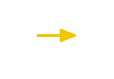
\begin{tikzpicture}[baseline]
    \node [anchor=base] (x) {};
    \draw [rawarrow] (x.mid west) -- ($(x.mid west) + (2em,0)$);
  \end{tikzpicture}
}

\newenvironment{slide}
{\begin{frame}[fragile,environment=slide]\vskip0pt plus 1filll}
{\vskip0pt plus 1filll\end{frame}}

% LaTeX

\setlength{\leftmargini}{1em}

% Common Information

\author{Talia Xu}
\course{COMPSCI 340}
\coursetitle{Operating Systems}
\date{2024 Semester 2}

% fontspec

\defaultfontfeatures{Ligatures=TeX}
% \setmainfont{Domine}
\setsansfont{Inter}[
  FontFace={ul}{n}{Font=*-Thin},
  FontFace={el}{n}{Font=*-ExtraLight},
  FontFace={l}{n}{Font=*-Light},
  FontFace={sb}{n}{Font=*-SemiBold},
  FontFace={eb}{n}{Font=*-ExtraBold},
  FontFace={xb}{n}{Font=*-Black},
]
\setmonofont[Contextuals=AlternateOff, Ligatures=TeXOff]{Iosevka}[
  FontFace={xb}{n}{Font=*-Heavy},
]

%% Font Weights

\DeclareRobustCommand{\ulseries}{\fontseries{ul}\selectfont}
\DeclareTextFontCommand{\textul}{\ulseries}
\DeclareRobustCommand{\elseries}{\fontseries{el}\selectfont}
\DeclareTextFontCommand{\textel}{\elseries}
\DeclareRobustCommand{\lseries}{\fontseries{l}\selectfont}
\DeclareTextFontCommand{\textl}{\lseries}
\DeclareRobustCommand{\sbseries}{\fontseries{sb}\selectfont}
\DeclareTextFontCommand{\textsb}{\sbseries}
\DeclareRobustCommand{\ebseries}{\fontseries{eb}\selectfont}
\DeclareTextFontCommand{\texteb}{\ebseries}
\DeclareRobustCommand{\xbseries}{\fontseries{xb}\selectfont}
\DeclareTextFontCommand{\textxb}{\xbseries}

% tikz

\usetikzlibrary{
  arrows,
  arrows.meta,
  automata,
  backgrounds,
  calc,
  decorations.pathreplacing,
  matrix,
  positioning,
  overlay-beamer-styles,
  shapes,
  shapes.multipart,
  tikzmark,
}

\tikzstyle{rawarrow} = [
  -{Latex[round]},
  line width=1pt,
  yellow,
  shorten >=3pt,
  shorten <=3pt,
  font=\small,
  text=black,
]

\tikzstyle{arrow} = [
  -{Latex[round]},
  line width=1pt,
  yellow,
  shorten >=3pt,
  shorten <=3pt,
  transform canvas={yshift=3pt},
  font=\small,
  text=black,
]

\newcommand{\tikzmarkcoord}[1]{([yshift=3pt]pic cs:#1)}

% minted

\setminted{style=eyolfson, fontsize=\small, escapeinside=||}
\setmintedinline{fontsize=\normalsize}

% hyperref

\hypersetup{colorlinks, urlcolor=blue}

% beamer
\setbeamersize{text margin left=16mm, text margin right=16mm}
\setbeamertemplate{itemize items}[circle]
\setbeamercolor{item}{fg=black}
\setbeamercolor{structure}{fg=darkblue}
\setbeamerfont{frametitle}{series=\bfseries, parent=structure}
\setbeamertemplate{navigation symbols}{}
\setbeamertemplate{headline}{}
\setbeamertemplate{footline}{
  \begin{tikzpicture}[
    remember picture,
    overlay,
    shift={(current page.south west)},
  ]
    \path [fill=gray] (144mm, 0) -- (160mm, 16mm) -- (160mm, 0);
    \node [inner sep=3.5mm, outer sep=0, text=black, anchor=base east,
           align=right, yshift=3.5mm]
          at (current page.south east) {\ttfamily \small \insertframenumber{}};
  \end{tikzpicture}
}
\setbeamertemplate{title page}{
  \begin{tikzpicture}[
    remember picture,
    overlay,
    shift={(current page.south west)},
    background rectangle/.style={fill=darkblue},
    show background rectangle,
  ]
    \node [anchor=center, align=center, text=white, text width=40mm, scale=3.2]
          at (\paperwidth / 2, \paperheight * 2 / 3)
          {\xbseries \inserttitle{}};
    \node [anchor=base west, align=left, inner sep=0, text=white, yshift=2.5mm]
          at (16mm, \paperheight / 3)
          {\insertdate{} \insertcourse{}: \insertcoursetitle{}};
    \node [anchor=base west, align=left, inner sep=0, text=white, yshift=-2.5mm]
          at (16mm, \paperheight / 3)
          {\insertauthor};
    \node [anchor=base east, align=right, inner sep=0, text=white, yshift=2.5mm]
          at (144mm, \paperheight / 3)
          {Lecture \insertlecturenumber{}};
    \node [anchor=base east, align=right, inner sep=0, text=white,
           yshift=-2.5mm]
          at (144mm, \paperheight / 3)
          {\ttfamily \insertversion{}};
    \node [align=center, anchor=south, inner sep=0, text=white, yshift=3.5mm]
          (license) at (\paperwidth / 2, 0)
          {\fontsize{7pt}{7pt}\selectfont This  work is licensed under a
           \href{http://creativecommons.org/licenses/by-sa/4.0/}
                {\color{lightblue} Creative Commons Attribution-ShareAlike 4.0
                 International License}};
  \end{tikzpicture}
}

% xcolor

%% Primary Colour

\definecolor{pantone655}{RGB}{0, 42, 92} % #002a5c
\colorlet{darkblue}{pantone655}

%% Secondary Colours

\definecolor{pantone633}{RGB}{0, 139, 176} % #008bb0
\colorlet{blue}{pantone633}

\definecolor{pantonewarmred}{RGB}{220, 70, 51} % #dc4633
\colorlet{red}{pantonewarmred}

\definecolor{pantone3285}{RGB}{0, 161, 137} % #00a189
\colorlet{cyan}{pantone3285}

\definecolor{pantone7722}{RGB}{13, 83, 77} % #0d534d
\colorlet{darkcyan}{pantone7722}

\definecolor{pantone376}{RGB}{141, 191, 46} % #8dbf2e
\colorlet{green}{pantone376}

\definecolor{pantone2613}{RGB}{109, 36, 122} % #6d247a
\colorlet{violet}{pantone2613}

\definecolor{pantone2985}{RGB}{111, 199, 234} % #6fc7ea
\colorlet{lightblue}{pantone2985}

\definecolor{pantone227}{RGB}{171, 19, 104} % #ab1368
\colorlet{magenta}{pantone227}

\definecolor{pantone7406}{RGB}{241, 197, 0} % #f1c500
\colorlet{yellow}{pantone7406}

%% Neutrals

\definecolor{pantonecoolgray2}{RGB}{208, 209, 201} % #d0d1c9
\colorlet{gray}{pantonecoolgray2}


\lecturenumber{34}
\title{Course Recap}
\version{2.0.0}

\begin{document}

\begin{frame}[plain, noframenumbering]
  \titlepage
\end{frame}

\begin{slide}
  
  \slidetitle{An Operating System Manages Resources}

  \centering

  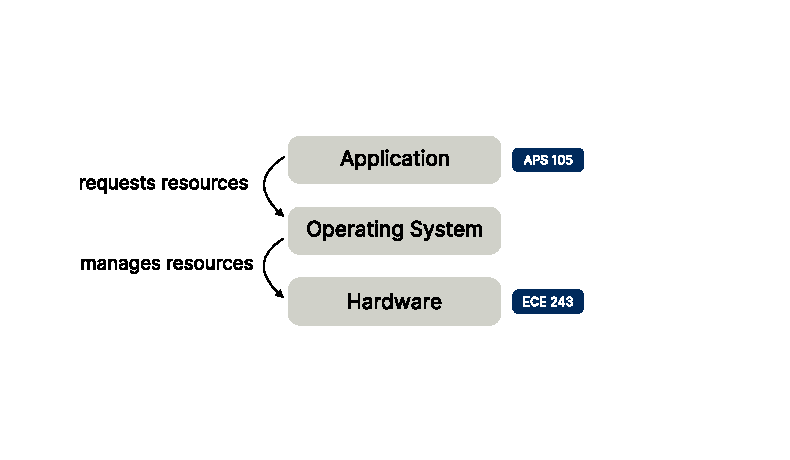
\includegraphics{../01-why-operating-systems/operating-system-overview.eps}

\end{slide}

\begin{slide}
  
  \slidetitle{There's 3 Core Operating System Concepts}

  \textbf{Virtualization:} share one resource by mimicking
  
  \leftspace{}multiple independent copies
  \bigskip

  \textbf{Concurrency:} handle multiple things happening at the same time
  \bigskip

  \textbf{Persistence:} retain data consistency even without power
\end{slide}

\begin{slide}
  
  \slidetitle{More Privileged CPU Modes Can Access More Instructions}

  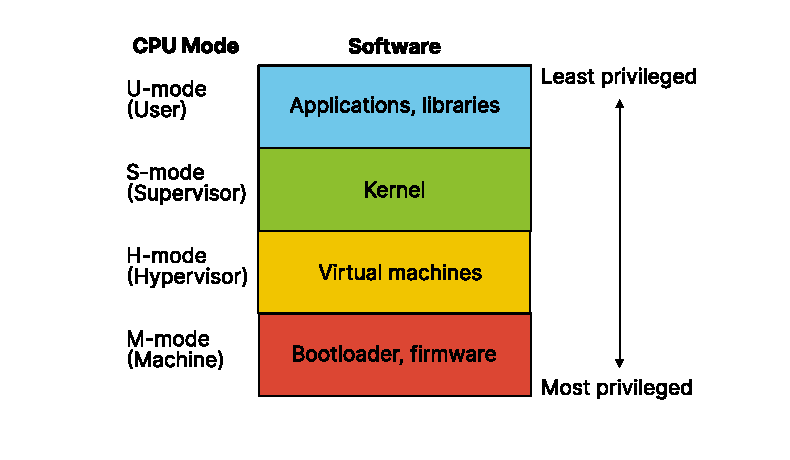
\includegraphics{../02-kernels/cpu-modes.eps}

\end{slide}

\begin{slide}
  
  \slidetitle{A Monolithic Kernel Runs Operating System Services in Kernel
              Mode}

  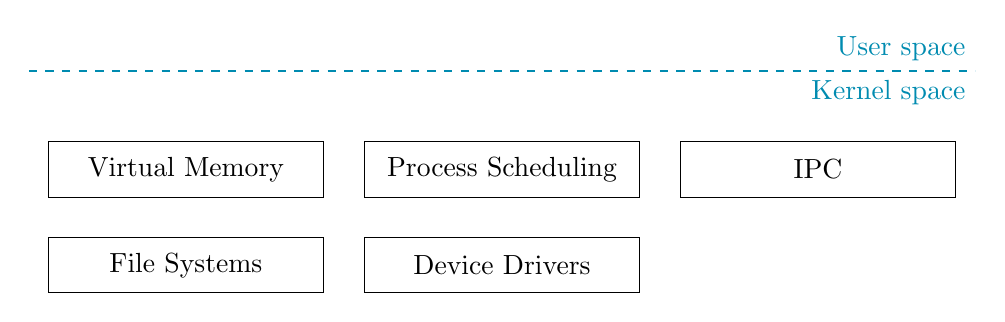
\begin{tikzpicture}[box/.style={draw, minimum width=3.5cm,
                                  minimum height=2em,
                                  inner sep=0.5em, node distance=0.5cm}]
    \draw [blue, dashed, thick] (0,0) -- ($(\textwidth - 3pt, 0)$);
    \node [blue, anchor=south east] at ($(\textwidth - 3pt, 0)$)
          (user) {User space};
    \node [blue, anchor=north east] at ($(\textwidth - 3pt, 0)$)
          (kernel) {Kernel space};
    \node [box] (sched) at ($(\textwidth/2 - 1.5pt, -1.25)$)
          {Process Scheduling};
    \node [box, left=of sched] {Virtual Memory};
    \node [box, right=of sched] {IPC};
    \node [box, below=of sched] (dd) {Device Drivers};
    \node [box, left=of dd] {File Systems};
  \end{tikzpicture}
\end{slide}

\begin{slide}
  
  \slidetitle{A Microkernel Runs the Minimum Amount of Services in Kernel
              Mode}

  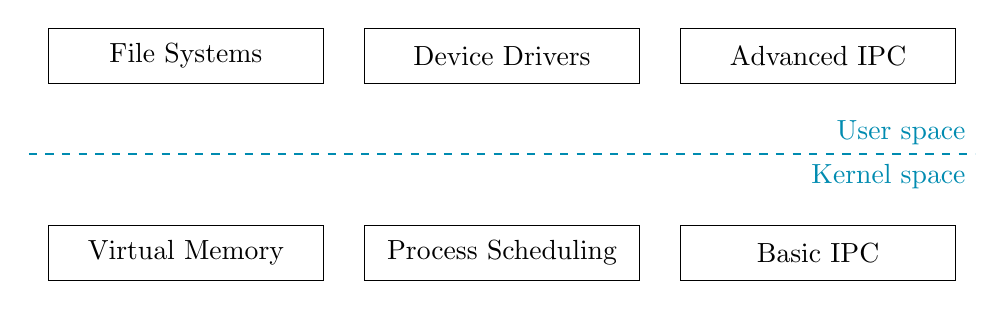
\begin{tikzpicture}[box/.style={draw, minimum width=3.5cm,
                                  minimum height=2em,
                                  inner sep=0.5em, node distance=0.5cm}]
    \draw [blue, dashed, thick] (0,0) -- ($(\textwidth - 3pt, 0)$);
    \node [blue, anchor=south east] at ($(\textwidth - 3pt, 0)$)
          (user) {User space};
    \node [blue, anchor=north east] at ($(\textwidth - 3pt, 0)$)
          (kernel) {Kernel space};
    \node [box] (sched) at ($(\textwidth/2 - 1.5pt, -1.25)$)
          {Process Scheduling};
    \node [box, left=of sched] {Virtual Memory};
    \node [box, right=of sched] {Basic IPC};
    \node [box] (dd) at ($(\textwidth/2 - 1.5pt, 1.25)$) {Device Drivers};
    \node [box, left=of dd] {File Systems};
    \node [box, right=of dd] {Advanced IPC};
  \end{tikzpicture}
\end{slide}

  \begin{slide}
    \slidetitle{Applications May Pass Through Multiple Layers of Libraries}

    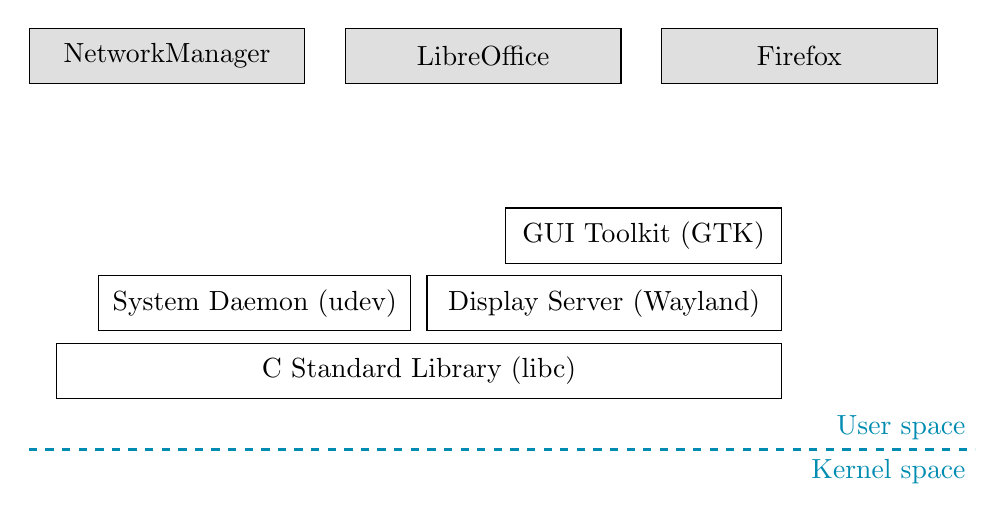
\begin{tikzpicture}[box/.style={draw, minimum width=3.5cm, minimum height=2em,
                                    inner sep=0.5em, node distance=0.5cm}]
      \draw [pantone633, dashed, thick] (0,0) -- ($(\textwidth - 3pt, 0)$);
      \node [pantone633, anchor=south east] at ($(\textwidth - 3pt, 0)$)
            (user) {User space};
      \node [pantone633, anchor=north east] at ($(\textwidth - 3pt, 0)$)
            (kernel) {Kernel space};

      \node [box, align=center, minimum width=9.2cm, xshift=-1cm] (libc) at ($(\textwidth/2 - 3pt, 1)$)
            {C Standard Library (libc)};

      \node [box, align=center, above=of libc, anchor=east, xshift=-0.1cm]
            {System Daemon (udev)};

      \node [box, align=center, above=of libc.north east, anchor=east, minimum width=4.5cm]
            (display) {Display Server (Wayland)};

      \node [box, above=of display.north east, anchor=east]
            {GUI Toolkit (GTK)};

      \node [box, fill=black!12.5,anchor=west] (app1) at (0, 5)
            {NetworkManager};

      \node [box, fill=black!12.5, right=of app1] (app2) {LibreOffice};

      \node [box, fill=black!12.5, right=of app2] {Firefox};
    \end{tikzpicture}
  \end{slide}

  \begin{slide}
    \slidetitle{The Operating System Creates Processes}

    The operating system has to:
    \begin{itemize}
      \item Maintain process control blocks, including state
      \item Create new processes
      \item Load a program, and re-initialize a process with context
    \end{itemize}

  \end{slide}

  \begin{slide}

    \slidetitle{You're Responsible for Managing Processes}

    The operating system maintains a strict parent/child relationship
    \medskip
    
    You should be able to identify (and prevent) the following:
    \begin{itemize}
      \item Zombie processes
      \item Orphan processes
    \end{itemize}
  \end{slide}

  \begin{slide}

    \slidetitle{We Explored Basic IPC in an Operating System}

    Some basic IPC includes:
    \begin{itemize}
      \item \texttt{read} and \texttt{write} through file descriptors (could be a regular file)
      \item Redirecting file descriptors for communcation
      \item Signals
    \end{itemize}
    \medskip

    Signals are like interrupts for user processes

    \leftspace{}The kernel has to handle all 3 kinds of ``interrupts''

  \end{slide}

  \begin{slide}

    \slidetitle{Scheduling Involves Trade-Offs}

    We looked at few different algorithms:

    \begin{itemize}
      \item First Come First Served (FCFS) is the most basic scheduling algorithm
      \item Shortest Job First (SJF) is a tweak that reduces waiting time
      \item Shortest Remaining Time First (SRTF) uses SJF ideas with preemptions
      \item SRTF optimizes lowest waiting time (or turnaround time)
      \item Round-robin (RR) optimizes fairness and response time
    \end{itemize}

  \end{slide}

  \begin{slide}

    \slidetitle{Scheduling Gets Even More Complex}

    There are more solutions, and more issues:

    \begin{itemize}
      \item Introducing priority also introduces priority inversion
      \item Some processes need good interactivity, others not so much
      \item Multiprocessors may require per-CPU queues
      \item Real-time requires predictability
      \item Completely Fair Scheduler (CFS) tries to model the ideal fairness
    \end{itemize}

  \end{slide}

  \begin{slide}

    \slidetitle{We Use Pages for Memory Translation}

    Divide memory into blocks, so we only have to translate once per block
    \medskip

    Use page tables (array of PTEs) to access the PPN (and flags)
    \medskip

    New problem: these page tables are always huge!

  \end{slide}

  \begin{slide}

    \slidetitle{Multi-Level Page Tables Save Space for Sparse Allocations}

    \centering
    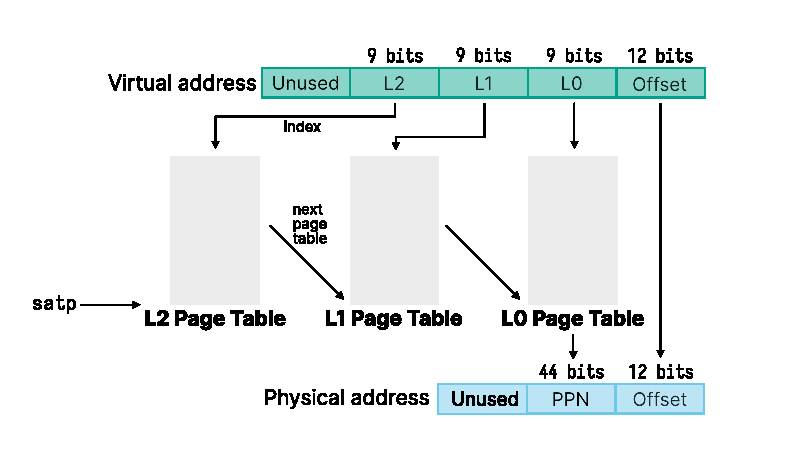
\includegraphics{../12-page-tables/multi-level-page-table.eps}

  \end{slide}

  \begin{slide}

    \slidetitle{Page Tables Translate Virtual to Physical Addresses}

    The MMU is the hardware that uses page tables, which may:

    \begin{itemize}
      \item Be a single large table (wasteful, even for 32-bit machines)
      \item Use the kernel allocated pages from a free list
      \item Be a multi-level to save space for sparse allocations
      \item Use a TLB to speed up memory accesses
    \end{itemize}

  \end{slide}

  \begin{slide}

    \slidetitle{We Had a Brief Detour}

    We explored a question using priority scheduling
    \medskip

    Also, we looked at \texttt{mmap} (not covered on the exam)

  \end{slide}

  \begin{slide}

    \slidetitle{Threads Enable Concurrency}

    We explored threads, and related them to something we already know (processes)

    \begin{itemize}
      \item Threads are lighter weight, and share memory by default
      \item Each process can have multiple threads (but just one at the start)
    \end{itemize}

  \end{slide}

  \begin{slide}

    \slidetitle{Both Processes and (Kernel) Threads Enable Parallelization}

    \begin{itemize}
      \item Each process can have multiple (kernel) threads
      \item Most implementations use one-to-one user-to-kernel thread mapping
      \item The operating system has to manage what happens during a fork, or signals
      \item We now have synchronization issues
    \end{itemize}

  \end{slide}

  \begin{slide}

    \slidetitle{Another Detour on Sockets, and \texttt{ucontext}}

    You don't have to know sockets for the exam, but they're just IPC
    \medskip

    \texttt{ucontext} is fair game (it's the state of the user registers)

  \end{slide}

  \begin{slide}
    \slidetitle{We Want Critical Sections to Protect Against Data Races}

    We should know what data races are, and how to prevent them:
    \begin{itemize}
      \item Mutex or spinlocks are the most straightforward locks
      \item We need hardware support to implement locks
      \item We need some kernel support for wake up notifications
      \item If we know we have a lot of readers, we should use a read-write lock
    \end{itemize}
  \end{slide}

  \begin{slide}

    \slidetitle{We Used Semaphores to Ensure Proper Order}

    Previously we ensured mutual exclusion, now we can ensure order

    \begin{itemize}
      \item Semaphores contain an initial value you choose
      \item You can increment the value using post
      \item You can decrement the value using wait (it blocks if the current
            value is 0)
      \item You still need to be prevent data races
    \end{itemize}

  \end{slide}

  \begin{slide}

    \slidetitle{We Explored More Advanced Locking}

    We have another tool to ensure order

    \begin{itemize}
      \item Condition variables are clearer for complex condition signaling
      \item Locking granularity matters
      \item You must prevent deadlocks
    \end{itemize}

  \end{slide}

  \begin{slide}
  
    \slidetitle{Disks Enable Persistence}
  
    We explored two topics: SSDs and RAID
  
    \begin{itemize}
      \item SSDs are more like RAM except accessed in pages and blocks
      \item SSDs also need to work with the OS for best performance (TRIM)
      \item Use RAID to tolerate failures and improve performance using multiple disks
    \end{itemize}
  
  \end{slide}

  \begin{slide}
    
    \slidetitle{Filesystems Enable Persistence}

    They describe how files are stored on disks:
    \begin{itemize}
      \item API-wise you can open files, and change the position to read/write
            at
      \item Each process has a local open file and there's a global open file
            table
      \item There's multiple allocation strategies: contiguous, linked, FAT, indexed
    \end{itemize}

  \end{slide}

  \begin{slide}
    
    \slidetitle{inodes Are a Hybrid Allocaiton Strategy}
    
    inodes are offer greater flexibility over: contiguous, linked, FAT, or
    indexed

    \begin{itemize}
      \item Everything is a file on UNIX, names in a directory can be hard or
            soft links
    \end{itemize}

  \end{slide}

  \begin{slide}

    \slidetitle{Page Replacement Algorithms Aim to Reduce Page Faults}

    We saw the following:
    \begin{itemize}
      \item Optimal (good for comparison but not realistic)
      \item Random (actually works surprisingly well, avoids the worst case)
      \item FIFO (easy to implement but Bélády's anomaly)
      \item LRU (gets close to optimal but expensive to implement)
    \end{itemize}

  \end{slide}

  \begin{slide}

    \slidetitle{The Clock Algorithm is an Approximation of LRU}

    Data structures:
    \begin{itemize}
      \item Keeps a circular list of pages in memory
      \item Uses a reference bit for each page in memory (light grey in next slides)
      \item Has a ``hand'' (iterator) pointing to the last element examined
    \end{itemize}
    \medskip

    Algorithm, to insert a new page:
    \begin{itemize}
      \item Check the hand's reference bit, if it's 0 then place the page and advance hand
      \item If the reference bit is 1, set it to 0, advance the hand, and repeat
    \end{itemize}
    \medskip

    For page accesses, set the reference bit to 1

  \end{slide}

  \begin{slide}

    \slidetitle{The Kernel Has To Implement It's Own Memory Allocations}

    The concepts are the same for user space memory allocation

    (the kernel just gives them more contiguous virtual memory pages):

    \begin{itemize}
      \item There's static and dynamic allocations
      \item For dynamic allocations, fragmentation is a big concern
      \item Dynamic allocation returns blocks of memory
        \begin{itemize}
          \item Fragmentation between blocks is external
          \item Fragmentation within a blocks is internal
        \end{itemize}
      \item There's 3 general allocation strategies for different sized
            allocations
        \begin{itemize}
          \item Best fit
          \item Worst fit
          \item First fit
        \end{itemize}
    \end{itemize}

  \end{slide}

  \begin{slide}

    \slidetitle{Even More Memory Allocations}
  
    The kernel restricts the problem for better memory allocation
    implementations
  
    \begin{itemize}
      \item Buddy allocator is a real-world restricted implementation
      \item Slab allocator takes advantage of fixed sized objects to reduce
            fragmentation
    \end{itemize}
  
  \end{slide}

  \begin{slide}
    
    \slidetitle{Virtual Machines Virtualize a Physical Machine}

    They allow multiple operating systems to share the same hardware

    \begin{itemize}
      \item Virtual machines provide isolation, the hypervisor allocates
            resources
      \item Type 2 hypervisors are slower due to trap-and-emulate and binary
            translation
      \item Type 1 hypervisors are supported by hardware, IOMMU speeds up devices
      \item Hypervisors may overcommit resources and need to physically move VM
      \item Containers aim to have the benefits of VMs, without the overhead
    \end{itemize}

  \end{slide}

  \begin{slide}

    \slidetitle{That's the Course!}

    Please let me know on Discord what you want me to review in our last lecture

  \end{slide}

\end{document}
